\chapter{Programming Assignment 2}

\begin{marginfigure}[5cm]
  \begin{center}
    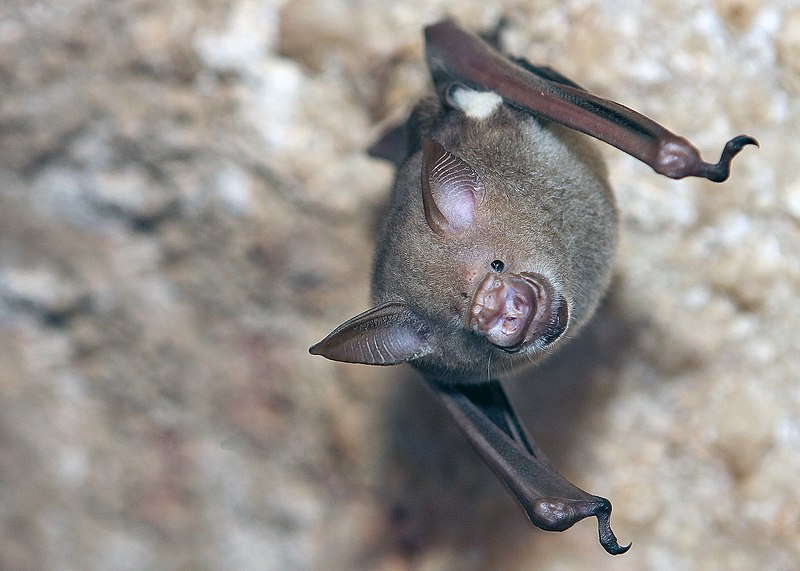
\includegraphics[width=\textwidth]{Assignments/figures/bat.jpg}
  \end{center}
  \caption{Bats use chirp-like ultrasound signals to sense their surroundings. Image: David Dennis.}
  \label{fig:bat_image}
\end{marginfigure}

This programming assignment deals with deconvolution of transmit
signals for an \emph{acoustic sounder} or a \emph{sonar}. A sonar is
a device that measures the amplitude of sound waves that are scattered
from objects at different propagation distances between the acoustic
wave transmitter and receiver. These devices are used, e.g., in cars to
assist with parking, in ships to measure the water depth, and for
non-invasive medical examinations. Sonars are also closely related
with radars, as they share many of the same signal processing
concepts. The main difference is that radars use electromagnetic waves
instead of acoustic waves.

In order to implement a simple sonar, I have used a loudspeaker and a
microphone connected to a sound card to transmit and receive acoustic
signals. The sampling rate of the audio recording is $f_s=44.1\cdot
10^3$ hertz. This setup allows me to also control what type of
signal is being transmitted. The loudspeaker and the microphone are
spaced apart by approximately 30 cm.
 
If we ignore measurement errors, the acoustic signal can be modeled using
a discrete-time convolution equation:
\begin{equation}
  m[n] = \sum_{r=0}^{R-1} h[r]x[n-r] = h[n] * x[n]
\end{equation}
In this equation $m[n]$ is the signal measured with a microphone,
$x[n]$ is the signal transmitted by the loudspeaker, and $h[n]$ is
the amplitude of the scattered signal as a function of range. The
signal $h[n]$ is also the impulse response of the space that the sonar
is measuring. The convolution equation can be motivated with a
range-time diagram that models the propagation of acoustic signals as
a function of range and time. Such a diagram is shown in Figure
\ref{fig:range_time_diagram_ex}.

\begin{figure}
\begin{center}
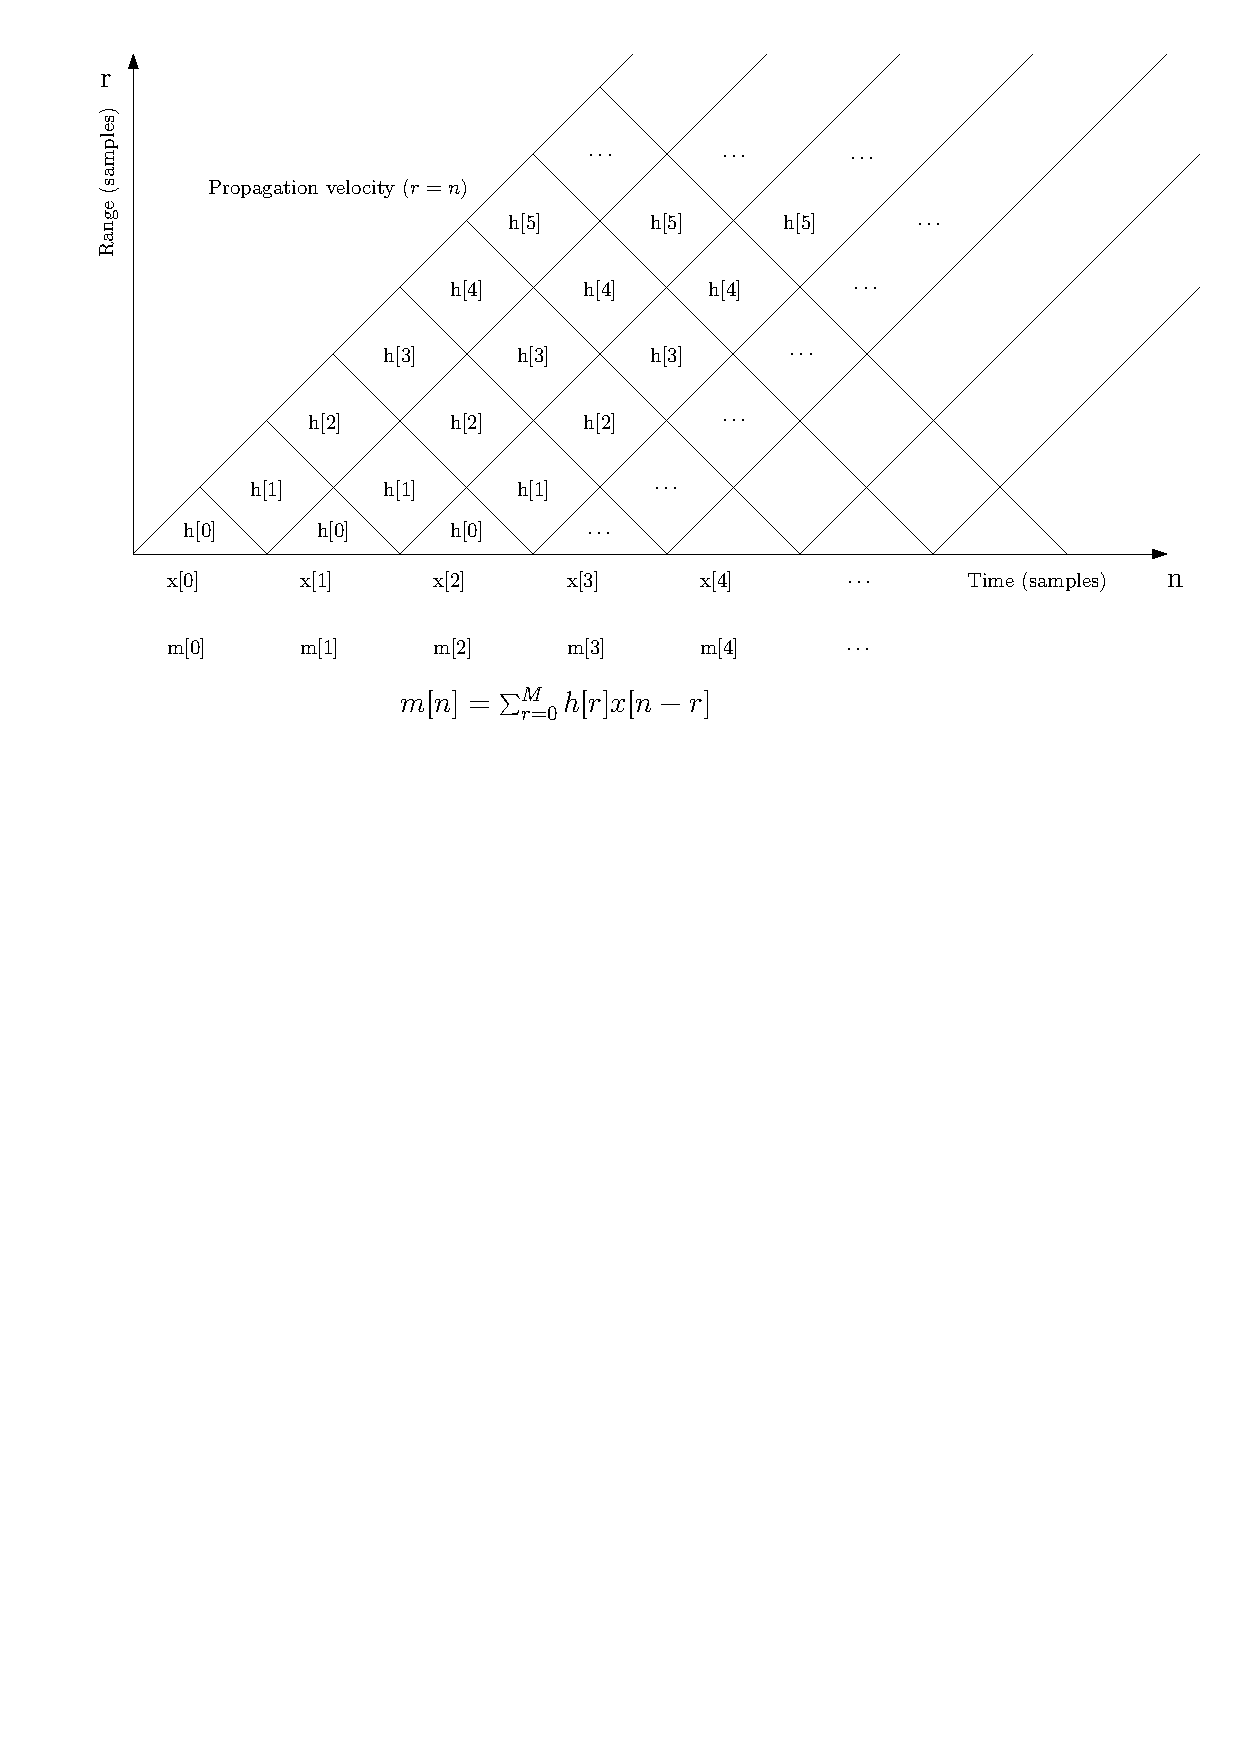
\includegraphics[width=\textwidth]{Applications/figures/rd.pdf}
\end{center}
\caption{A range-time diagram depicting the relationship between a transmitted signal and a scattered signal.}
\label{fig:range_time_diagram_ex}
\end{figure}

Modern sonars often use long waveforms in order to compress more
energy into the transmitted pulse without increasing the amount of
peak power. Longer waveforms also make it easier to separate multiple
different transmitters from one another, reducing interference. 

One of the main objectives of a sonar measurement is to recover the impulse
response $h[n]$ from measurements $m[n]$. This is trivial when the
transmit pulse is a unit impulse $x[n]=A\delta[n]$. With longer
transmit signals, we need to deconvolve the transmitted signal. This
is typically achieved by convolving the received signal $m[n]$ with a deconvolution filter $\lambda[n]$:
\begin{equation}
  \lambda[n]*m[n] = \lambda[n] * x[n] * h[n].
\end{equation}
The deconvolution filter needs to have the following property\sidenote{One way to determine $\lambda[n]$ is to solve for it in frequency domain, but this is beyond the scope of this exercise.}:
\begin{equation}
  \lambda[n]*x[n] \approx A\delta[n],
\end{equation}
where $A$ is a constant. In the case of chirp-like signals, an often used deconvolution filter is the time reversed chirp signal:
\begin{equation}
  \lambda[n] = x[-n + n_0],
\end{equation}
where $n_0$ is a suitable time shift. 

For this assignment, I have used an amplitude tapered chirp-like waveform
of the following form:
\begin{equation}
  x[n] = \left\{
\begin{array}{ccc}
  \sin^2\left(\frac{\pi n}{N}\right) \sin(2\pi \beta T_s^2 n^2) & \mathrm{when} & 0 \le n < N\\
  0 & \mathrm{otherwise} & 
  \end{array}\right.
\end{equation}
Here $N$ is the integer length of the chirp pulse in samples and
$\beta = \frac{1}{2 N T_s}f_{\mathrm{max}}$ is the chirp-rate, which
determines how fast the instantaneous frequency of the signal
increases as a function of time. Figure \ref{fig:tx_pulse_chirp} shows
this waveform with $N=1000$ and $\beta = 486202.5\ \text{s}^{-2}$.     

\begin{marginfigure}
  \begin{center}
    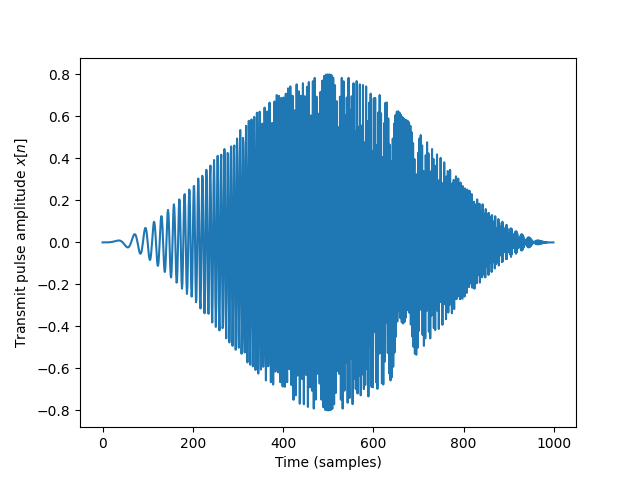
\includegraphics[width=\textwidth]{Assignments/figures/chirp_tx.png}
  \end{center}
  \caption{The chirp transmit pulse signal $x[n]$ used for this exercise.
    In this case, the pulse is $N=1000$ samples long, sweeping in frequency between 0 and 22.05 kHz.}
  \label{fig:tx_pulse_chirp}
\end{marginfigure}

You will need to download two data files for this task:
\begin{itemize}
  \item \url{http://kaira.uit.no/juha/chirp.bin}
  \item \url{http://kaira.uit.no/juha/sonar_meas.bin}
\end{itemize}
The first one contains the transmitted chirp waveform $x[n]$ and the second one
contains a microphone recording during a sonar experiment $m[n]$. Note that
if you do not want to use the provided recordings, feel free to use
your own sonar setup. You will need a microphone and a loudspeaker, and
some software that will transmit the chirp waveform in a loop. You can
also borrow my equipment in order to make your own measurements.

You can read these signals into a
computer as follows:
\begin{lstlisting}[language=Python,numbers=none]
import numpy as n
import matplotlib.pyplot as plt

# read chirp waveform
chirp=n.fromfile("chirp.bin",dtype=n.float32)
# read microphone recording 
m=n.fromfile("sonar_meas.bin",dtype=n.float32)

plt.plot(chirp)
plt.xlabel("Time (samples)")
plt.ylabel("Transmitted signal $x[n]$")
plt.show()

# plot the first three interpulse periods 
plt.plot(m[0:30000])
plt.xlabel("Time (samples)")
plt.ylabel("Received signal $m[n]$")
plt.show()
\end{lstlisting}
These acoustic pulses are transmitted every $M=10000$ samples. This
means that the sonar is repeating a measurement of $h[n]$ every
$10000$ samples and the transmitted signal actually looks like this:
\begin{equation}
  \epsilon[n] = \sum_{k=0}^{N_p-1} x[n - Mk]
\end{equation}
In this task, you should treat each segment of 10000 samples as an
independent sonar measurement, which will allow you to study how the
impulse response evolves over time. You can do this as follows:
\begin{lstlisting}[language=Python,numbers=none]
import numpy as n
import matplotlib.pyplot as plt

m=n.fromfile("sonar_meas.bin",dtype=n.float32)

interpulse_period=10000
N_ipps = int(n.floor(len(m)/interpulse_period))
for i in range(N_ipps):
    echoes = m[(i*interpulse_period):(i*interpulse_period+interpulse_period)]
    plt.plot(echoes)
    plt.show()

    # convolve echo with deconvolution filter
    # deconvolved = n.convolve(echo,deconvolution_filter,mode="same")
\end{lstlisting}
In this listing I have also added a hint for you on how you can
implement the deconvolution operation $A h[n] \approx
\lambda[n]*m[n]$ for each interpulse period consisting of 10000 samples.

For this assignment, you are to perform the following tasks. Write a
short report describing what you did and what results you got. The
report is otherwise free form, as long as it is in PDF format. Include
your code and plots in the report. 

You will find a lot of help for this task in the lecture notes that
discusses LTI systems, convolution and frequency response. You may
help each other on Perusall. It is fine to give hints, but please try
not to give away the \emph{exact solution}.

\begin{enumerate}[a)]
\item How many meters of distance\sidenote{I mean total distance, \emph{not half the total distance}, which is often used in sonar and radar to take into account the fact that the wave has to travel to the target and back.} does an acoustic pulse travel during one sample duration $T_s = f_s^{-1}$? Assume sound speed in a typical lecture room at UiT.

  \item How long is the transmitted pulse read from file \verb|chirp.bin| in seconds?  

  \item How long is the measurement in seconds? You can figure this out by looking at the length of the signal \verb|sonar_meas.bin| and using the known sample-rate of $44.1 \cdot 10^3$ samples per second.
    
  \item How many transmit pulses are contained in the measurement? One
    pulse is transmitted every 10000 samples.
    
 \item Why does the deconvolution filter $\lambda[n]$ need to have the
  property: $\lambda[n]*x[n] \approx A\delta[n]$, where $A$ is a
  constant?
   
 \item Evaluate the autocorrelation function of the transmitted signal
   $c[n]=x[n]*x[-n-n_0]$. Use the signal that you read from
   \verb|chirp.bin|. You can time-reverse a signal in Python using
   \verb|deconvolution_filter = x[::-1]|. Make a plot of $c[n]$
   zooming into the portion of the signal that has significantly
   non-zero values.

 \item How close is $c[n]$ in your opinion to a scaled unit
   impulse $A\delta[n]$? How will deviations from the unit impulse
   affect deconvolution quality when using $\lambda[n]=x[-n-n_0]$ as a
   deconvolution filter?

 \item Make a plot of the scattered power as a function of time and
   range. Use one pulse for each column of the array that you are
   plotting.  You should get something similar to the plot in Figure
   \ref{fig:ex_rti_plot}. Use decibel scale for power. Use time in
   seconds on the x-axis and total propagation distance in meters on
   the y-axis. Total propagation distance means the total travelled
   distance between the loudspeaker and the microphone. You can use,
   e.g., the \verb|pcolormesh| command from Python's Matplotlib to
   make this plot.

  \begin{figure}
  \begin{center}
    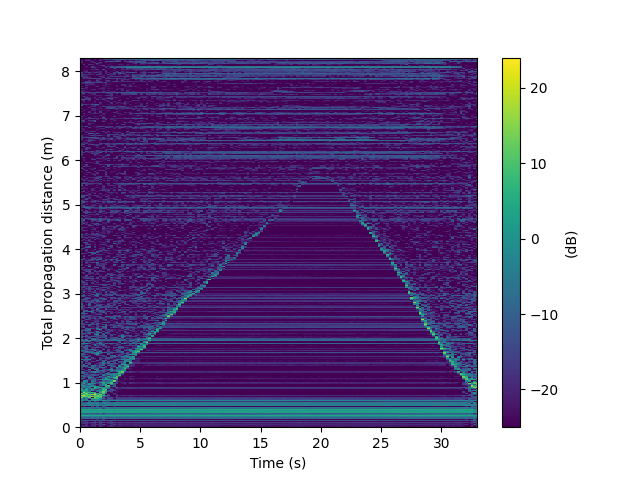
\includegraphics[width=\textwidth]{Assignments/figures/sonar_rti.png}
  \end{center}
  \caption{An example range-time intensity plot showing how much power
    in decibel scale is scattered back from the surroundings of the
    sonar system. The distance between the microphone and the
    loudspeaker is about 30 cm, which can be seen as a constant
    horizontal line at the propagation distance. The plot also shows an
    acoustic scatterer that is first moving away and then moving back
    towards the transmitter.}
  \label{fig:ex_rti_plot}
\end{figure}

\end{enumerate}
